\subsection{Base de Datos}

Modelo entidad-relación de la base de datos que será utilizada para la
aplicación TREEBAR. Se tendrán las tablas observadas en las
Figuras~\ref{fig:reseñas} y~\ref{fig:certificaciones}, utilizando además
la API de BARCODE LOOKUP de la que se obtendrá la información relevante 
de los productos .

\begin{figure}[H]
    \centering
    \fbox{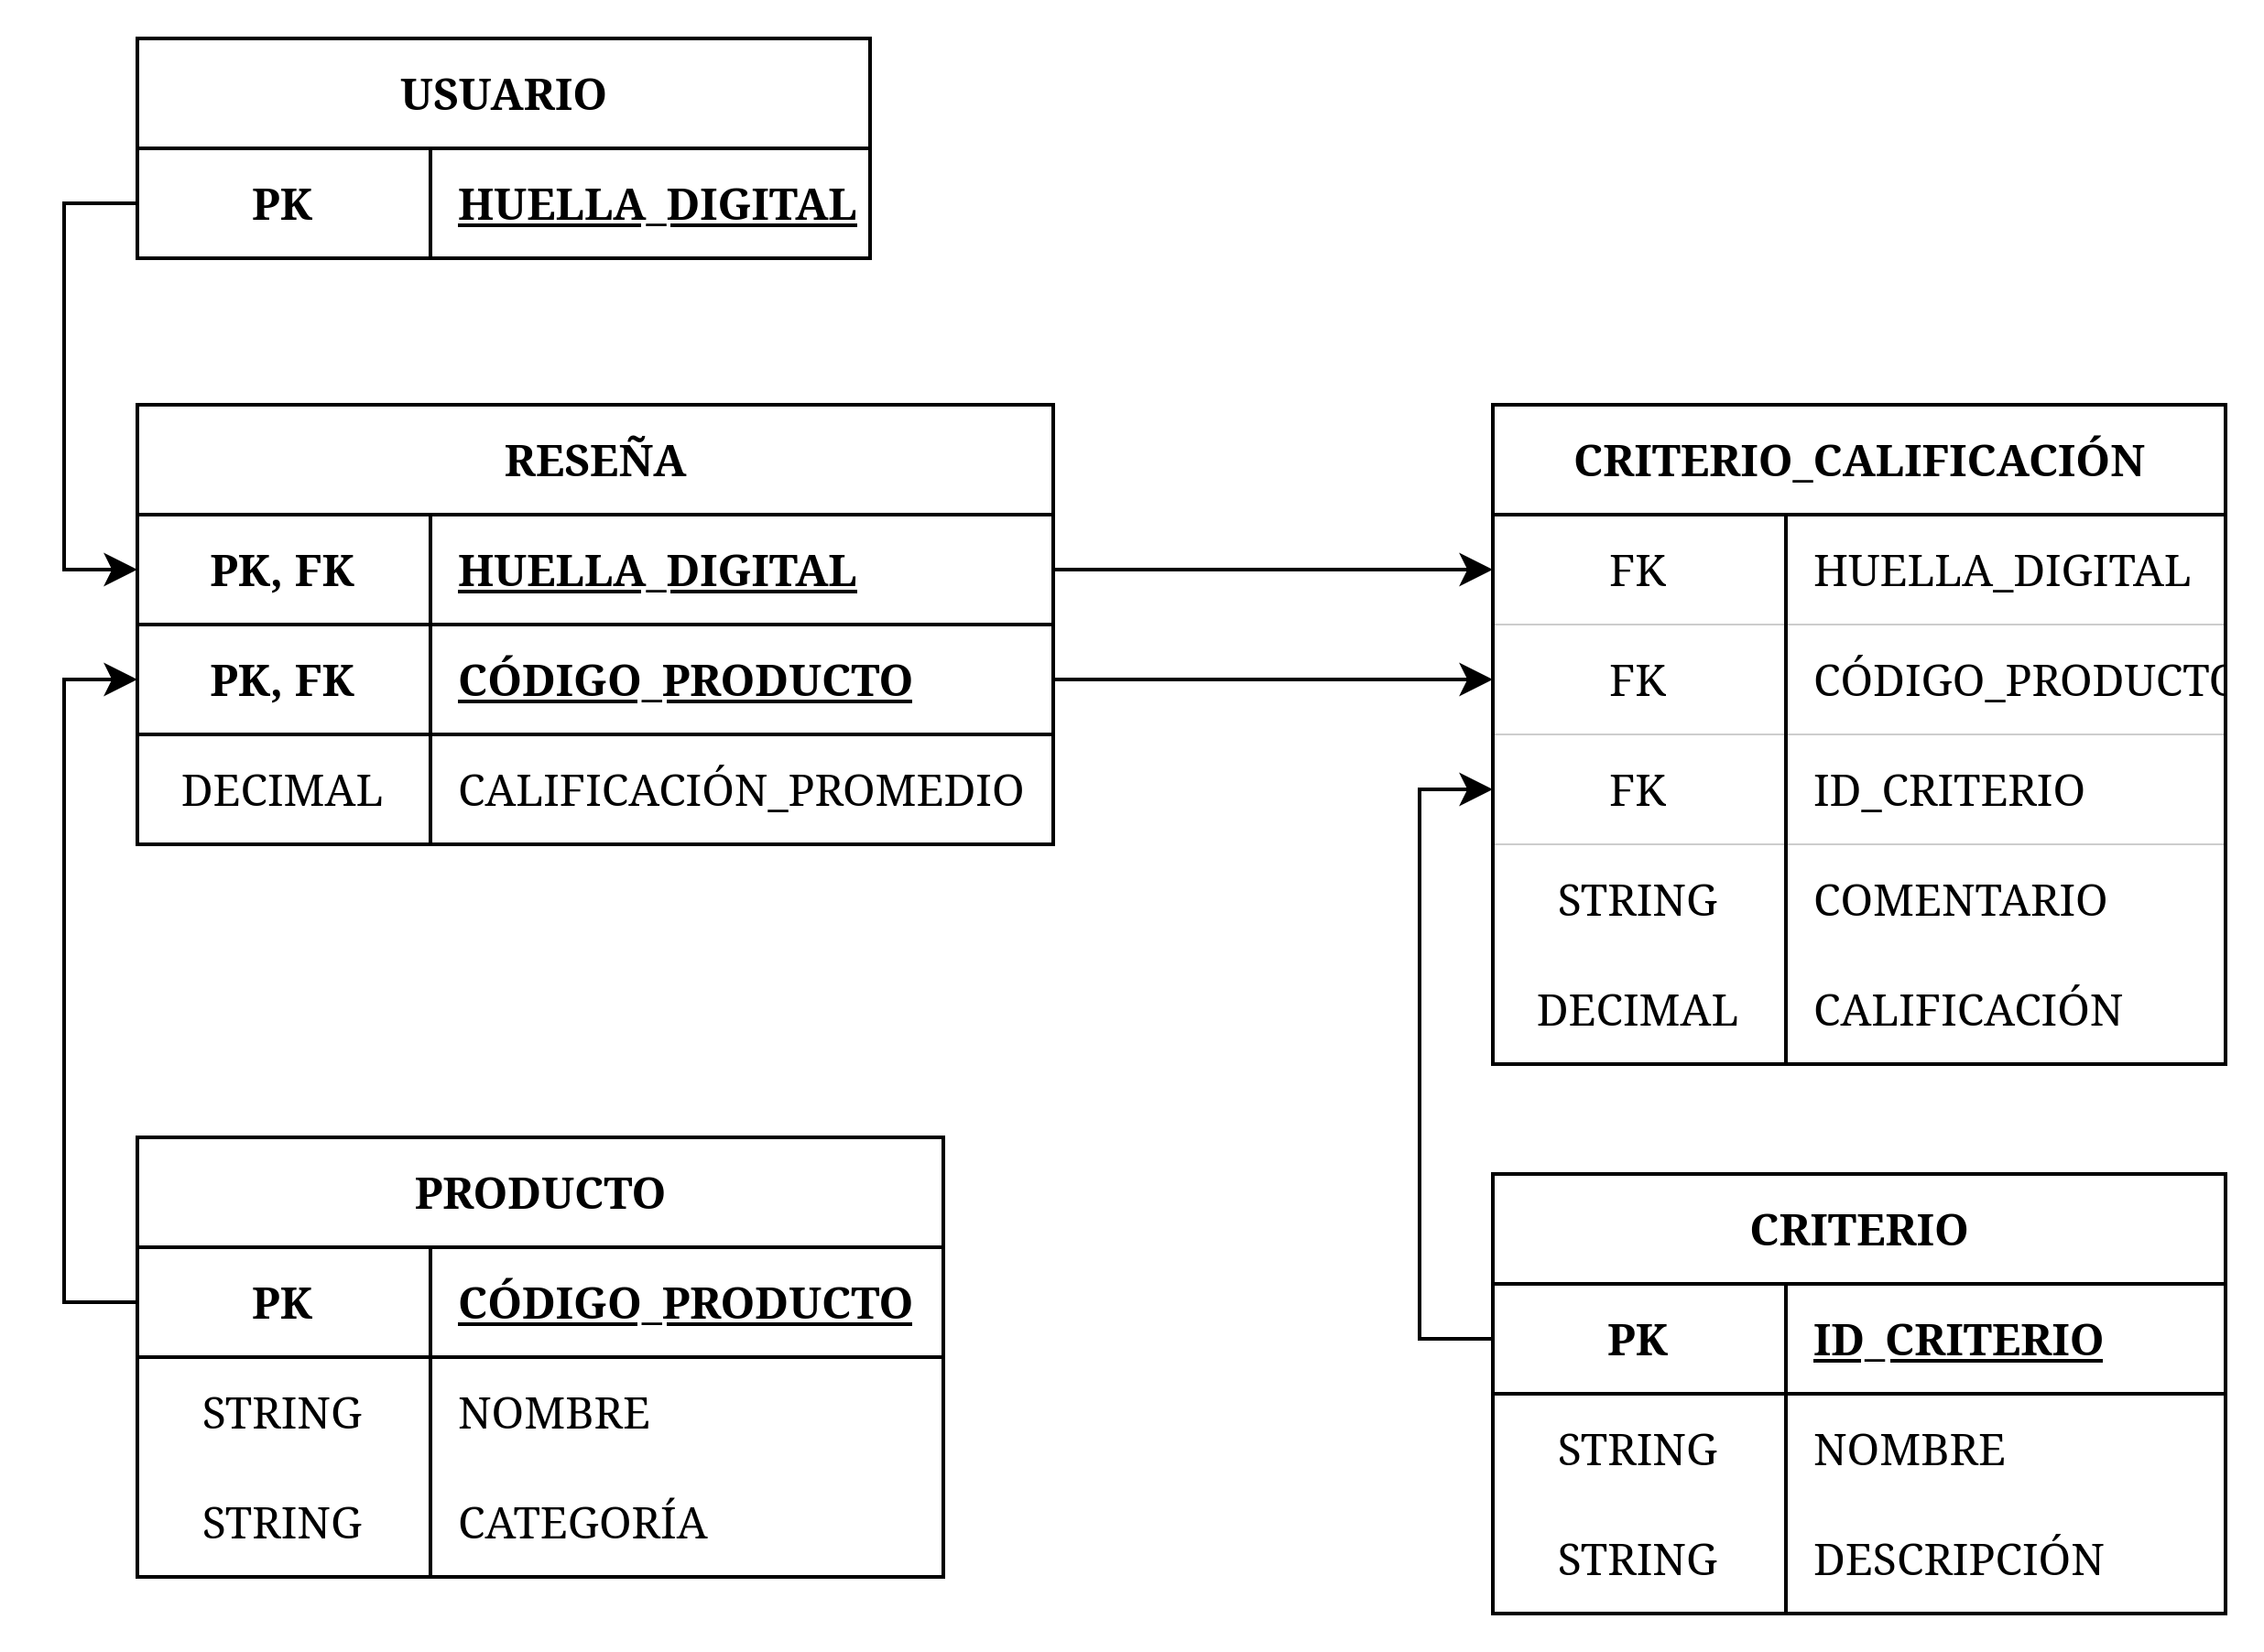
\includegraphics[width=0.8\textwidth]{imagenes/reseñas.png}}
    \caption{Relación de las tablas que contienen información proporcionada por
    el usuario en relación a la calidad de los productos.}\label{fig:reseñas}
\end{figure}

\begin{figure}[H]
    \centering
    \fbox{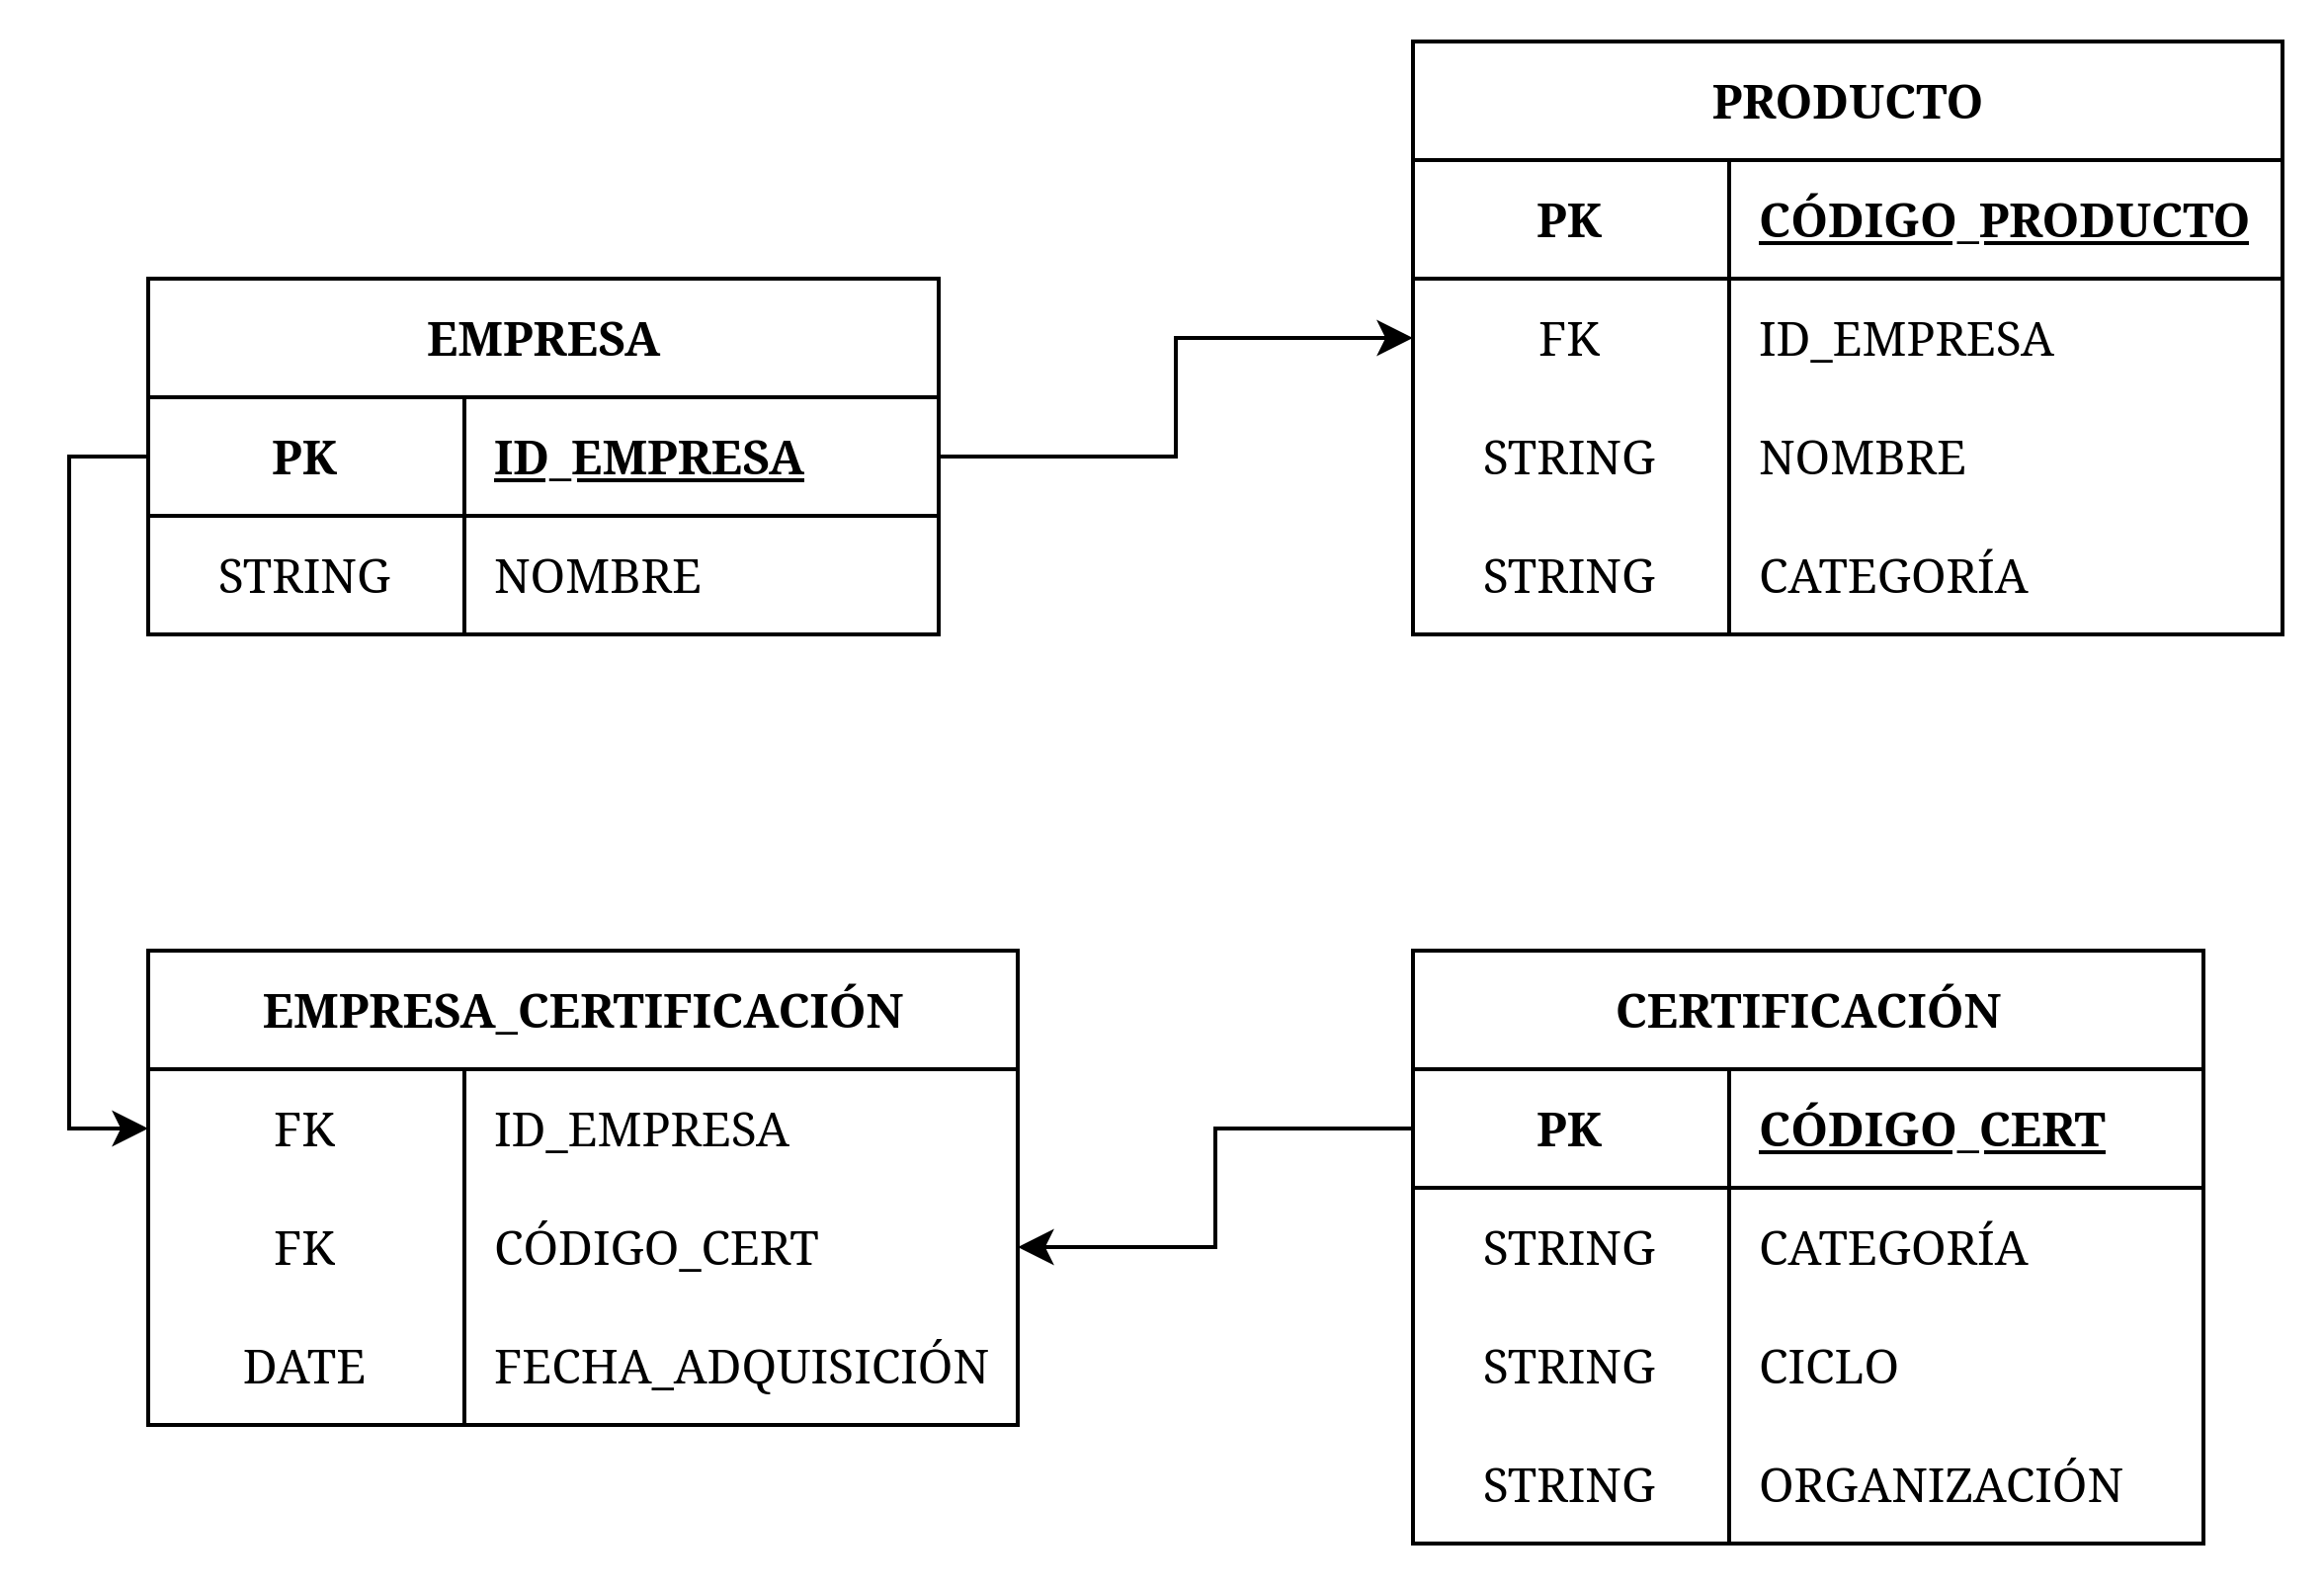
\includegraphics[width=0.8\textwidth]{imagenes/certificaciones.png}}
    \caption{Relación de las tablas que muestran la información pertinente de
    las empresas propietarias de los productos.}\label{fig:certificaciones}
\end{figure}